% =====================================================================
% AI Academy -- National AI Center
% Software Engineering Final Project -- Team Presentation Deck
% =====================================================================

\PassOptionsToPackage{dvipsnames}{xcolor}
\documentclass[aspectratio=169,11pt]{beamer}

% ===== CONFIGURATION ====================================
\newcommand{\teamname}{M503}
\newcommand{\topicchoice}{Topic 4 --- Async Research Assistant}
\newcommand{\memberone}{Orkhan Nuriyev (@orxannuriyev)}
\newcommand{\membertwo}{Nazrin Burziyeva (@nazrinburz)}
\newcommand{\memberthree}{Gunel Garayzade (@gunelrafig)}
\newcommand{\repolink}{github.com/orxannuriyev/research\_assistant}

\newcommand{\coursecode}{AI-ENG-503}
\newcommand{\coursename}{Software Engineering}
\newcommand{\institution}{AI Academy, National AI Center}
\newcommand{\semester}{Autumn 2026}

% ===== PACKAGES ======================================================
\usepackage[T1]{fontenc}
\usepackage[utf8]{inputenc}
\usepackage{xcolor}
\usepackage{tabularx}
\usepackage{booktabs}
\usepackage{listings}
\usepackage{tikz}
\usetikzlibrary{shapes.geometric,arrows.meta,positioning,fit,backgrounds}

% ===== EARLY MACROS ==================================================
\definecolor{accent2}{HTML}{8B0000}
\newcommand{\TODO}[1]{\textcolor{accent2}{\textbf{[TODO: #1]}}}

% ===== BEAMER THEME =================
\usetheme{default}
\usefonttheme{professionalfonts}
\setbeamertemplate{navigation symbols}{}

\definecolor{accent}{HTML}{0B3D91}
\definecolor{soft}{HTML}{F2F4F8}
\definecolor{ok}{HTML}{166534}

\setbeamercolor{title}{fg=accent}
\setbeamercolor{frametitle}{fg=accent}
\setbeamercolor{section in head/foot}{bg=accent,fg=white}
\setbeamercolor{itemize item}{fg=accent}
\setbeamercolor{itemize subitem}{fg=accent}
\setbeamercolor{enumerate item}{fg=accent}
\setbeamercolor{block title}{bg=accent,fg=white}
\setbeamercolor{block body}{bg=soft,fg=black}

\setbeamerfont{title}{size=\Large,series=\bfseries}
\setbeamerfont{frametitle}{size=\large,series=\bfseries}
\setbeamerfont{footline}{size=\tiny}

% Footer with team + slide number
\setbeamertemplate{footline}{%
  \leavevmode%
  \hbox{\hspace*{2ex}\tiny\textit{\teamname{} -- \topicchoice}\hfill%
  \tiny\textit{\coursecode{} -- \semester{}}\hfill%
  \tiny\insertframenumber/\inserttotalframenumber\hspace*{2ex}}%
  \vskip1pt%
}

% ===== CODE LISTINGS =================================================
\definecolor{codegreen}{rgb}{0,0.55,0}
\definecolor{codepurple}{rgb}{0.55,0,0.78}
\lstdefinestyle{python}{
  language=Python,
  backgroundcolor=\color{soft},
  commentstyle=\color{codegreen},
  keywordstyle=\color{accent},
  stringstyle=\color{codepurple},
  basicstyle=\ttfamily\scriptsize,
  breaklines=true,
  frame=single,
  framerule=0.4pt,
  rulecolor=\color{black!30},
}

% =====================================================================
\begin{document}

% ========== SLIDE 1: TITLE ===========================================
{%
\setbeamertemplate{footline}{}
\begin{frame}[plain]
  \begin{center}
    \vspace{0.6cm}
    {\small \textsc{\institution}}\\[0.2em]
    {\small \textsc{\coursecode{} -- \coursename{} -- \semester{}}}\\[1.2em]
    \rule{0.7\textwidth}{0.6pt}\\[0.4em]
    {\Huge\bfseries\color{accent} \topicchoice}\\[0.4em]
    \rule{0.7\textwidth}{0.6pt}\\[1.2em]
    {\large \teamname}\\[0.6em]
    {\normalsize \memberone\quad\textbullet\quad\membertwo\quad\textbullet\quad\memberthree}\\[1cm]
    {\footnotesize\itshape Final Project Defense -- 2026-09-19}\\[0.4em]
    {\footnotesize\texttt{\repolink}}
  \end{center}
\end{frame}
}

% ========== SLIDE 2: PROBLEM =========================================
\begin{frame}{The problem in one sentence}
  \begin{block}{What the system does}
    A user asks a natural-language question; we query Wikipedia, arXiv, and Web concurrently, and return a single synthesised answer with numbered inline citations.
  \end{block}

  \vspace{0.3em}
  \begin{columns}[T,onlytextwidth]
  \column{0.48\textwidth}
  \textbf{Inputs}
  \begin{itemize}
    \item Natural-language question ($\le$500 chars)
    \item Target source list (e.g. wiki, arxiv, web)
  \end{itemize}

  \column{0.48\textwidth}
  \textbf{Outputs}
  \begin{itemize}
    \item Synthesised answer text
    \item Numbered references used (title, url)
  \end{itemize}
  \end{columns}

  \vspace{0.4em}
  \textbf{Entry points:} CLI (\texttt{python -m researcher ask}) \& HTTP API (\texttt{POST /research})
\end{frame}

% ========== SLIDE 3: ARCHITECTURE ====================================
\begin{frame}{Architecture}
  \textbf{Module map.} The boundary between the \emph{provided} \texttt{ai/} package and \emph{our} SE layer is shown explicitly.

  \vspace{0.3em}
  \begin{center}
  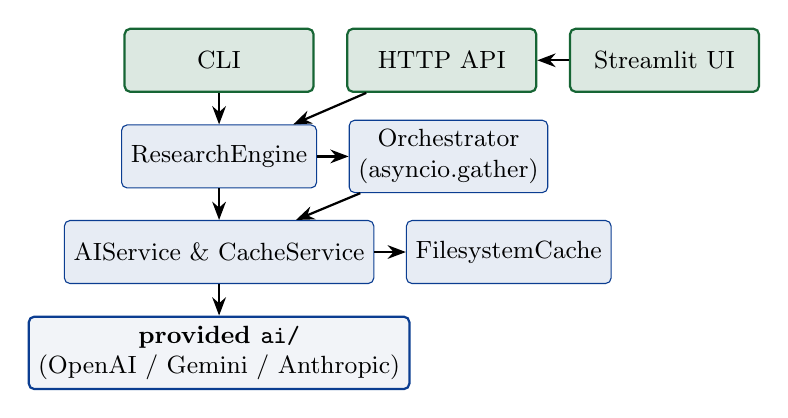
\begin{tikzpicture}[
    node distance=4mm,
    box/.style={draw,rounded corners=2pt,minimum width=2.4cm,minimum height=0.8cm,align=center,font=\small},
    aibox/.style={box,fill=soft,draw=accent,thick},
    sebox/.style={box,fill=accent!10,draw=accent},
    entry/.style={box,fill=ok!15,draw=ok,thick},
    arrow/.style={-Stealth,thick}
  ]
    % Entry points
    \node[entry] (cli) {CLI};
    \node[entry,right=of cli] (api) {HTTP API};
    \node[entry,right=of api] (ui) {Streamlit UI};

    % SE layer
    \node[sebox,below=of cli] (core) {ResearchEngine};
    \node[sebox,right=of core] (conc) {Orchestrator\\(asyncio.gather)};
    \node[sebox,below=of core] (svc)  {AIService \& CacheService};
    \node[sebox,right=of svc] (store) {FilesystemCache};

    % AI module
    \node[aibox,below=of svc] (ai) {\textbf{provided \texttt{ai/}}\\(OpenAI / Gemini / Anthropic)};

    % Arrows
    \draw[arrow] (cli) -- (core);
    \draw[arrow] (api) -- (core);
    \draw[arrow] (ui) -- (api);
    \draw[arrow] (core) -- (conc);
    \draw[arrow] (core) -- (svc);
    \draw[arrow] (conc) -- (svc);
    \draw[arrow] (svc) -- (ai);
    \draw[arrow] (svc) -- (store);
  \end{tikzpicture}
  \end{center}

  \vspace{0.3em}
  {\footnotesize\textit{ResearchEngine coordinates the concurrent fetching via Orchestrator and the final synthesis via AIService.}}
\end{frame}

% ========== SLIDE 4: KEY DESIGN DECISIONS ============================
\begin{frame}{Three design decisions we can defend}
  \begin{enumerate}\setlength\itemsep{0.6em}
    \item \textbf{asyncio over threads}\\
      The workload is purely I/O-bound (network latency); threads have higher memory overhead and GIL contention.
    \item \textbf{Filesystem JSON cache over SQLite}\\
      Atomic JSON writes (temp file + \texttt{os.replace}) prevent corruption and are trivial to inspect during debugging.
    \item \textbf{Pydantic Settings over manual env parsing}\\
      Provides built-in type casting, defaults, and validation for our 12 configuration variables with a single \texttt{Settings} singleton.
  \end{enumerate}

  \vspace{0.6em}
\end{frame}

% ========== SLIDE 5: CONCURRENCY (THE BENCHMARK) =====================
\begin{frame}{Concurrency: the benchmark}
  \textbf{Workload:} benchmark query across the three source adapters; Wikipedia returned 403 in the recorded run.

  \vspace{0.4em}
  \begin{center}\small
  \begin{tabular}{lcc}
    \toprule
    & \textbf{Sequential} & \textbf{Concurrent (sem=5)} \\
    \midrule
    Wall-clock (s) & 3.03 & 2.38 \\
    Speedup        & 1.0$\times$ & \textbf{1.28$\times$} \\
    Provider 429s  & 0  & 0 \\
    \bottomrule
  \end{tabular}
  \end{center}

  \vspace{0.4em}
  \textbf{Bottleneck named:} arXiv's mandatory 1s polite interval limits parallel gains.\\
  \textbf{What didn't reach $3\times$:} The final LLM synthesis step is fundamentally sequential, and the arXiv lock limits throughput.

  \vspace{0.3em}
  {\footnotesize\textit{Numbers run on Windows, Python 3.11 via \texttt{python scripts/bench.py}.}}
\end{frame}

% ========== SLIDE 6: ROBUSTNESS STORY ================================
\begin{frame}{Robustness: one concrete failure mode}
  \textbf{Scenario:} Wikipedia intermittently returned HTTP 403 Forbidden due to IP blocking.

  \vspace{0.3em}
  \textbf{How we surfaced it:} During live testing of the concurrent fetch pipeline.

  \vspace{0.3em}
  \textbf{What the system does:}
  \begin{itemize}\setlength\itemsep{0.3em}
    \item \textbf{Retry:} Tenacity retries HTTP 4xx (non-429) errors up to 3 times with exponential backoff.
    \item \textbf{Log:} \texttt{WARNING source 'wikipedia' failed: 403 Forbidden -- skipping.}
    \item \textbf{Degrade:} \texttt{asyncio.gather} receives empty results for Wikipedia.
    \item \textbf{Validate:} The engine successfully synthesises an answer using only arXiv and Web without crashing.
  \end{itemize}
\end{frame}

% ========== SLIDE 7: DEMO ============================================
\begin{frame}[fragile]{Live demo}
  \begin{block}{What we will run}
    An offline question answering pipeline using mock AI endpoints and cached sources.
  \end{block}

  \vspace{0.4em}
  \textbf{Demo command (works inside Docker):}
  \begin{lstlisting}[style=python,language=bash,numbers=none]
$ docker run --rm finalproj
$ docker run --rm --env-file .env finalproj \
    python -m researcher ask "What is CRISPR?" --sources wiki,arxiv
\end{lstlisting}

  \vspace{0.4em}
  \begin{itemize}
    \item Outputs a cohesive markdown-styled answer with numbered citations.
    \item CLI correctly respects the \texttt{--sources} filter and \texttt{--no-cache} flags.
  \end{itemize}

  \vspace{0.3em}
  {\footnotesize\textit{HTTP endpoint also available via \texttt{POST /research}.}}
\end{frame}

% ========== SLIDE 8: TESTING =========================================
\begin{frame}{Testing}
  \begin{columns}[T,onlytextwidth]
  \column{0.55\textwidth}
  \textbf{Coverage \& shape}
  \begin{itemize}\setlength\itemsep{0.3em}
    \item Total \texttt{src/} coverage: \textbf{86\%}
    \item Provided \texttt{ai/} smoke tests: \textcolor{ok}{\textbf{passing}}
    \item Test count: 51 passed
    \item All tests offline; AI module fully mocked
  \end{itemize}

  \column{0.42\textwidth}
  \textbf{Three tests worth calling out}
  \begin{itemize}\setlength\itemsep{0.3em}
    \item Happy-path end-to-end integration
    \item Concurrency source failure isolation
    \item Cache TTL expiry catches timezone bugs
  \end{itemize}
  \end{columns}

  \vspace{0.6em}
  \begin{block}{Tooling}
    \texttt{pytest} + \texttt{pytest-cov} + \texttt{unittest.mock}.
  \end{block}
\end{frame}

% ========== SLIDE 9: LIMITATIONS + FUTURE ============================
\begin{frame}{Limitations \& what we'd do next}
  \textbf{Where the system is brittle today}
  \begin{itemize}\setlength\itemsep{0.3em}
    \item No multi-provider failover; if the selected provider is down, we return no answer.
    \item arXiv's 1s lock caps throughput severely on large concurrent batches.
    \item Cache staleness is TTL-based; no event-driven invalidation.
  \end{itemize}

  \vspace{0.4em}
  \textbf{Given another week we would}
  \begin{enumerate}\setlength\itemsep{0.3em}
    \item Add automatic fallback between configured LLM providers.
    \item Implement a Token-Bucket rate limiter for arXiv to allow bursts.
    \item Stream LLM tokens via \texttt{async for} for better perceived UI latency.
  \end{enumerate}
\end{frame}

% ========== SLIDE 10: TEAM CONTRIBUTIONS =============================
\begin{frame}{Team contributions}
  \begin{center}\small
  \begin{tabularx}{\linewidth}{lXl}
    \toprule
    \textbf{Member} & \textbf{Primary ownership} & \textbf{Workload} \\
    \midrule
    Orkhan Nuriyev   & Core orchestration, storage, config   & 2642 added, 16 deleted, 5 commits \\
    Nazrin Burziyeva & Service integration, CLI, tests, Docker & 1278 added, 542 deleted, 13 commits \\
    Gunel Garayzade  & Initial AI/API integration, Streamlit UI, provider selection, Swagger & 1395 added, 373 deleted, 6 commits \\
    \bottomrule
  \end{tabularx}
  \end{center}

  \vspace{0.4em}
  \textbf{Collaborative integration:} Gunel established the initial AI/API integration, completed the Streamlit UI and provider selection, and contributed PR~\#15's bilingual UI/API iteration; Nazrin completed the surrounding engine and service integration, robustness, tests, and Docker packaging.

  \vspace{0.4em}
  \textbf{AI tool use:} \textit{AI scaffolded API routes and tests; we refactored OOP structure, fixed timezone bugs, and wrote edge-case tests.}
\end{frame}

% ========== SLIDE 11: THANK YOU / Q&A ================================
{%
\setbeamertemplate{footline}{}
\begin{frame}[plain]
  \begin{center}
    \vspace{1cm}
    {\Huge\bfseries\color{accent} Questions?}\\[1.2em]
    \rule{0.5\textwidth}{0.6pt}\\[1.2em]
    {\large \teamname}\\[0.6em]
    {\normalsize \texttt{\repolink}}\\[1cm]
    {\footnotesize\itshape ``We can walk through any file in the repo.''}
  \end{center}
\end{frame}
}

\end{document}
